\documentclass[final]{lmuposter}
% helpful for justifying the boxes, use the following in the header:
%
\setlength{\parindent}{0pt}

% German language
%\usepackage[ngerman]{babel}
% Fonts of package UTF8
\usepackage[utf8x]{inputenc}

% pgf and tikz for graphics
\usepackage{pgf}
\usepackage{pgflibrarysnakes}
\usepackage{tikz}

% mathematical symbols of the ams package
\usepackage{amsmath}
\usepackage{amssymb}
\usepackage{bbm}

% supfigures
\usepackage{subfig}

% macros for vectors, matrix and so on
\newsavebox{\fmbox}
\newenvironment{fmpage}[1]
	{\begin{lrbox}{\fmbox}\begin{minipage}{#1}}
	{\end{minipage}\end{lrbox}\fbox{\usebox{\fmbox}}}
%
% Puts a algorithm environment
\newenvironment{algorithm}[1][]{%
	\begin{table}[h]
	\centering
	\begin{minipage}[t]{12cm}
	\hspace{\stretch{2}} {\caption{\label{#1} #1}}
	\rule[1.5ex]{12cm}{0.01cm}\\
	%\hspace{\stretch{2}} {\tiny \textsc{ #1}}}
	\hspace{\stretch{2}} \\
	% SPACE BEFORE \\ IS IMPORTANT, ELSE NO STRETCHING
	\vspace{-4ex}
	\begin{list}{#1}{\labelwidth=12em \leftmargin=120pt}
	\vspace{-1ex}
}{%
	\end{list}
	\rule[1ex]{12cm}{0.01cm}\\
	\end{minipage}
	\vspace{-2ex}
	\end{table}
}
%
\newcommand{\atem}[2]{\item[\texttt{#1}] #2\vspace{1ex}}
%
% Some math stuff, you need to include \usepackage{amsmath} 
%
%
%\mathop is needed to  get the spacing correct,
%
\newcommand{\sign}{\mathop{\mathrm{sign}}}
%
% greek symbols are displayed fat, too 
%
\renewcommand{\vector}[1]{\boldsymbol{#1}}
%
% use straight letters for matrixes
%
\renewcommand{\matrix}[1]{\mathbf{#1}}
%
% Some further definitions
%
\newcommand{\set}[1]{\mathbb{#1}}
\newcommand{\transpose}{\mathsf{T}}
\newcommand{\unity}{\mathbbm{1}}

\usepackage{MnSymbol}

% multicols package
\usepackage{multicol}

% Python source code highlighting. Uses the listings package. Use lstinputlistings in the boxes of the
% poster.
% Python listing setup
\usepackage{color}
\usepackage[procnames]{listings}
\usepackage{setspace}
\renewcommand{\lstlistlistingname}{Code Listings}
\renewcommand{\lstlistingname}{Code Listing}
\definecolor{gray}{gray}{0.5}
\definecolor{lightgray}{gray}{0.9}
\definecolor{green}{rgb}{0,0.5,0}
\definecolor{lightgreen}{rgb}{0,0.7,0}
\definecolor{orange}{rgb}{1,0.5,0}
\definecolor{purple}{rgb}{0.5,0,0.5}
\definecolor{darkred}{rgb}{0.5,0,0}


\lstset{
language=python,
extendedchars=true,
%basicstyle=\ttfamily\small\setstretch{1},
basicstyle=\footnotesize,
mathescape=true,
breaklines=true,
numbers=left,
numbersep=10pt,
numberstyle=\tiny,
framexleftmargin=30pt,
xleftmargin=55pt,
stringstyle=\color{green},
showstringspaces=false,
alsoletter={1234567890},
otherkeywords={\ , \}, \{},
keywordstyle=\color{blue},
emph={access,and,as,break,class,continue,def,del,elif,else,%
except,exec,finally,for,from,global,if,import,in,is,%
lambda,not,or,pass,print,raise,return,try,while,assert},
emphstyle=\color{orange}\bfseries,
emph={[2]self},
emphstyle=[2]\color{gray},
emph={[4]ArithmeticError,AssertionError,AttributeError,BaseException,%
DeprecationWarning,EOFError,Ellipsis,EnvironmentError,Exception,%
False,FloatingPointError,FutureWarning,GeneratorExit,IOError,%
ImportError,ImportWarning,IndentationError,IndexError,KeyError,%
KeyboardInterrupt,LookupError,MemoryError,NameError,None,%
NotImplemented,NotImplementedError,OSError,OverflowError,%
PendingDeprecationWarning,ReferenceError,RuntimeError,RuntimeWarning,%
StandardError,StopIteration,SyntaxError,SyntaxWarning,SystemError,%
SystemExit,TabError,True,TypeError,UnboundLocalError,UnicodeDecodeError,%
UnicodeEncodeError,UnicodeError,UnicodeTranslateError,UnicodeWarning,%
UserWarning,ValueError,Warning,ZeroDivisionError,abs,all,any,apply,%
basestring,bool,buffer,callable,chr,classmethod,cmp,coerce,compile,%
complex,copyright,credits,delattr,dict,dir,divmod,enumerate,eval,%
execfile,exit,file,filter,float,frozenset,getattr,globals,hasattr,%
hash,help,hex,id,input,int,intern,isinstance,issubclass,iter,len,%
license,list,locals,long,map,max,min,object,oct,open,ord,pow,property,%
quit,range,raw_input,reduce,reload,repr,reversed,round,set,setattr,%
slice,sorted,staticmethod,str,sum,super,tuple,type,unichr,unicode,%
vars,xrange,zip},
emphstyle=[4]\color{purple}\bfseries,
morecomment=[s][\color{lightgreen}]{"""}{"""},
morekeywords={and,as,assert,break,class,continue,def,del,elif,else,except,
     finally,for,from,global,if,import,in,is,lambda,not,or,pass,print,
     return,try,while,with,yield},
commentstyle=\color{red}\slshape,
%literate={>>>}{\textbf{\textcolor{darkred}{>{>}>}}}3%
%         {...}{{\textcolor{gray}{...}}}3,
procnamekeys={def,class},
procnamestyle=\color{blue}\textbf,
%framexleftmargin=0mm, framextopmargin=0mm, frame=ovalbox,
backgroundcolor=\color{lightgray},
frame=single,
framerule=0pt,
}



% Bibliography.
\usepackage[numbers,sort&compress, square]{natbib}
%
% Remove the bibliography header.
%
\makeatletter
\renewenvironment{thebibliography}[1]{%
%     \section*{\refname}%
%      \@mkboth{\MakeUppercase\refname}{\MakeUppercase\refname}%
      \list{\@biblabel{\@arabic\c@enumiv}}%
           {\settowidth\labelwidth{\@biblabel{#1}}%
            \leftmargin\labelwidth
            \advance\leftmargin\labelsep
            \@openbib@code
            \usecounter{enumiv}%
            \let\p@enumiv\@empty
            \renewcommand\theenumiv{\@arabic\c@enumiv}}%
      \sloppy
      \clubpenalty4000
      \@clubpenalty \clubpenalty
      \widowpenalty4000%
      \sfcode`\.\@m}
     {\def\@noitemerr
       {\@latex@warning{Empty `thebibliography' environment}}%
      \endlist}
\makeatother

% some modifications for the lists environment
%\renewcommand{\labelitemii}{$\blacktriangleright$}%
\setlength{\itemsep}{1mm}
\setlength{\parsep}{1mm}

\begin{document}
\nocite{obspy}

%
% Document header
%
\PosterHead{
	\textbf{\LARGE ObsPy: A Python Toolbox for Seismology/Seismological Observatories}\\[0.4ex]
	\textit{\Large Interactive Application and Rapid Program Development} \\[0.5ex]
	\large \underline{Lion Krischer}$^{\text{a}}$, Moritz Beyreuther$^{\text{a}}$, Robert Barsch$^{\text{a}}$, Tobias Megies$^{\text{a}}$, Yannik Behr$^{\text{b}}$, Joachim Wassermann$^{\text{a}}$\\
	$^{\text{a}}$ LMU Munich \hspace{2em}  $^{\text{b}}$ Victoria University of Wellington, New Zealand\\
	Department of Earth and Environmental Sciences (Geophysics), Ludwig-Maximilians-University Munich, Germany\\
	Contact: \textit{krischer@geophysik.uni-muenchen.de}, \textbf{http://www.obspy.org}
}

%
%\renewcommand{\capsize}{\footnotesize}
%
\setlength{\columnsep}{\MyBoxHSep}
\vspace{-1.5em}
\begin{multicols}{2}

%
% First box. Top left.
%
\MyBox[8em]{

\section*{Abstract}
\textbf{Python} enables the user to combine the advantages of a fully grown programming language with the flexibility of an interactive scripting language. Its extensive standard library and many freely available high quality scientific modules enable rapid development.

\textbf{ObsPy} provides the ability to read and write many common waveform file formats as well as seismological signal processing routines.

Furthermore \textbf{NumPy} (numpy.scipy.org) and \textbf{SciPy} (scipy.org) offer a wide variety of numerical multidimensional array programming methods. Together with \textbf{IPython} (ipython.scipy.org) and \textbf{Matplotlib} (matplotlib.sourceforge.net) ObsPy offers a powerful, text-based and easy to learn interactive environment consisting of free software packages.

ObsPy has a \textbf{modular architecture} which aims at minimizing the dependencies and is available under the \textbf{GPL/LGPLv3} licences.
}\vspace{\MyBoxVSep}


%
% Second box.
%
\MyBox[8em]{

\section*{Reading and Writing}
ObsPy provides unified access to read and write most commonly used waveform formats such as \textbf{MiniSEED, GSE2, SAC, SEISAN and the Seismic Handler formats Q and ASCII}. All data is stored in a Stream object consisting of multiple Traces of contiguous time series. Every Trace keeps track of its own meta information and the data is available as \textbf{numpy.ndarrays}.

% Code for reading.
\lstinputlisting[firstline=1, lastline=5]{code/reading.py}

The Stream and Trace objects have many built-in methods, like filtering and plotting:
\lstinputlisting[firstline=7, lastline=7, firstnumber=6]{code/reading.py}

\begin{center}
\begin{tikzpicture}
\node[above right,text width=0.9\textwidth]at(0cm,0cm){ 
\tiny
\centering
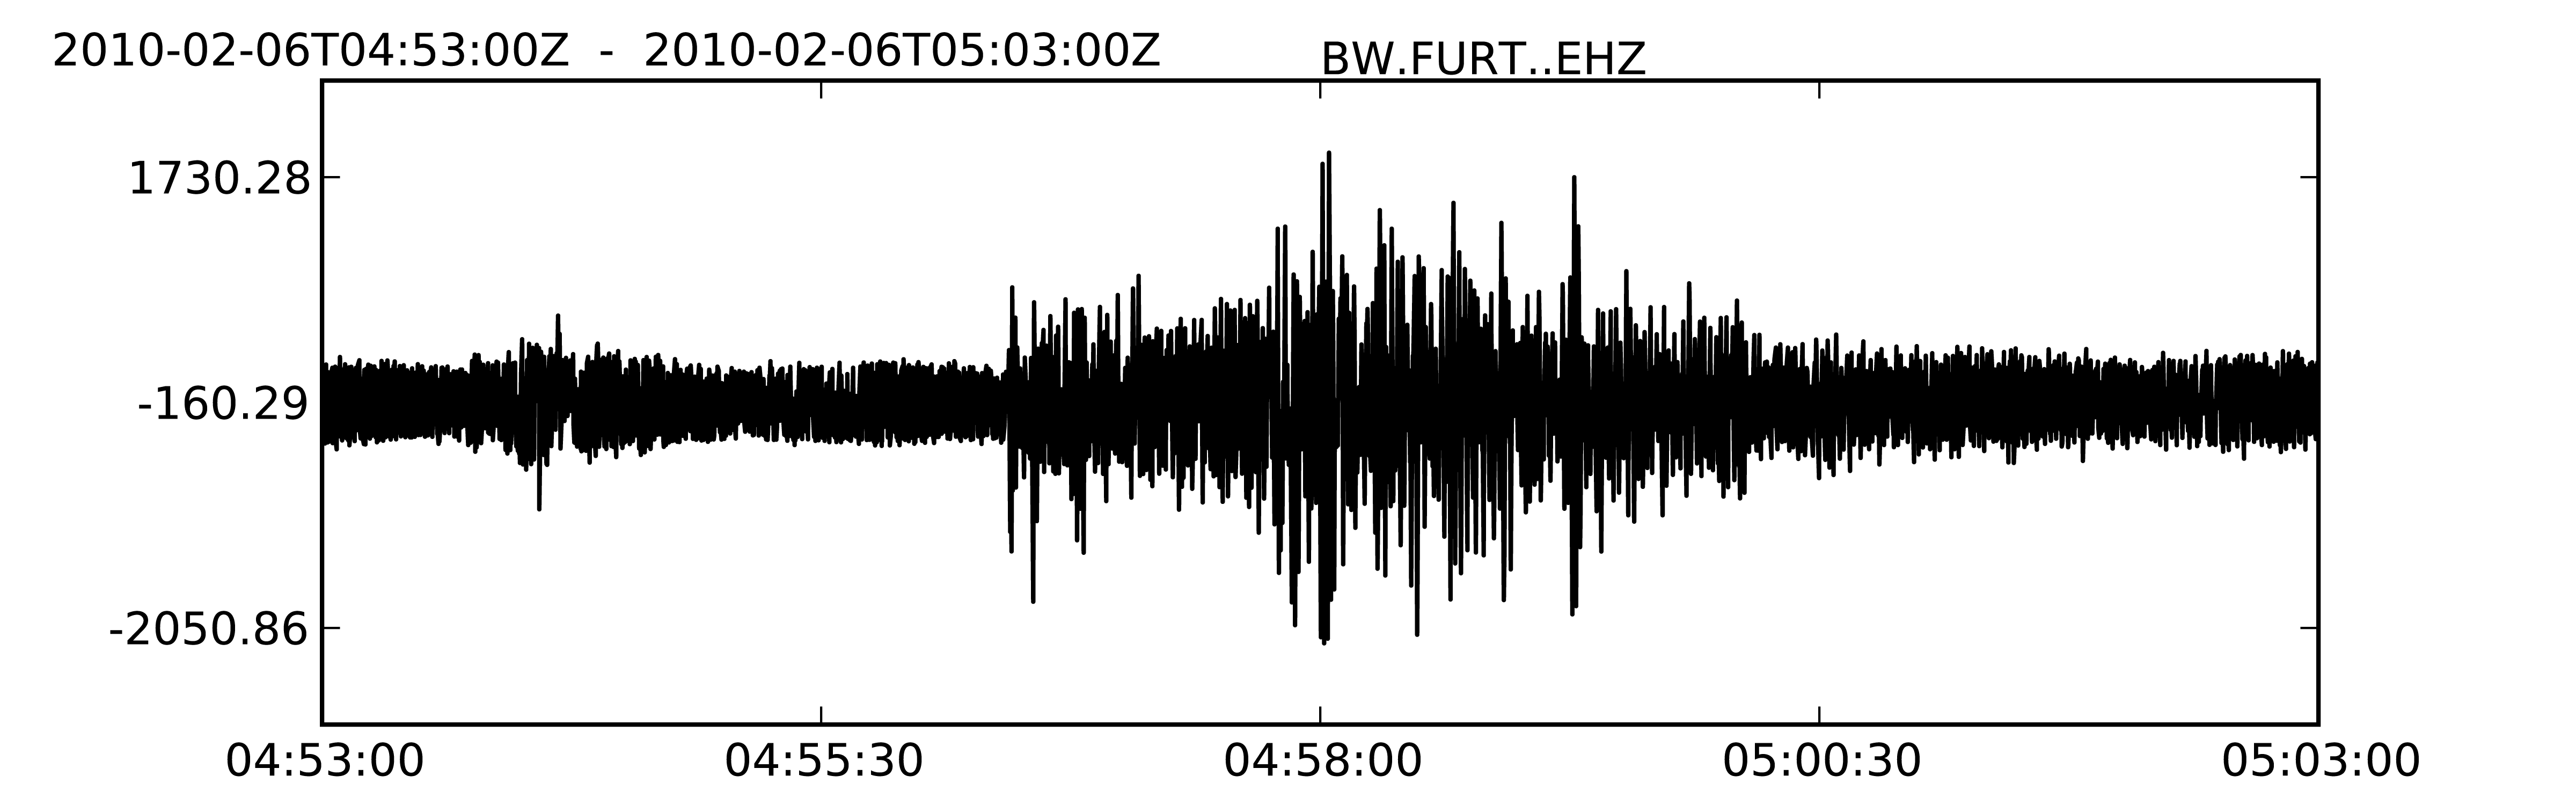
\includegraphics[width=0.9\textwidth]{simple_plot}\\[-3ex]
};
\end{tikzpicture}
{\newline \small \textbf{Figure~1}: Graphical representation of the Stream object. Created with obspy.imaging.
} \\[.5\MyBoxVSep]
\end{center}

\vspace{2ex}
Data can be exported with the write method.
\lstinputlisting[firstline=9, lastline=9, firstnumber=7]{code/reading.py}


}\vspace{\MyBoxVSep}

\MyBox[8em]{

\section*{Data Retrieval}
ObsPy also has support to retrieve data from ArcLink (www.webdc.eu), Fissures (www.iris.edu/dhi) and SeisHub (www.seishub.org)\citep{seishub}:\\
\newline
\vspace{-2ex}
\lstinputlisting[firstline=7, lastline=10, firstnumber=1]{code/arclink.py}
}\vspace{\MyBoxVSep}

\columnbreak%\\

%
% Third box.
%
\MyBox[8em]{
\section*{SEED/XML-SEED Support}
XML-SEED \citep{xseed} is a XML representation of the Dataless SEED format \citep{seed}. ObsPy is able to convert SEED
\lstinputlisting{code/seed_example.py}
to XML-SEED and back and furthermore it can extract RESP files from either format.
\lstinputlisting[firstline=2, lastline=5]{code/xseed_example.py}
\textbf{obspy.xseed} is, to the authors' knowledge, the only freely available and working implementation of XML-SEED.

}\vspace{\MyBoxVSep}

%
% Fourth box.
%

\MyBox[8em]{
\begin{multicols}{2}
\section*{obspy.signal}
Various processing routines, for example:
\vspace{-2ex}
\subsection*{Instrument Correction}
This example shows the correction of a STS2 to a 1 Hz seismometer using \textbf{obspy.signal}.
\newline
The data is read with \textbf{obspy.core}, then the mean value is subtracted.
\lstinputlisting[firstline=8, lastline=9, firstnumber=9]{code/korrektur.py}
Now the data is corrected with the simulate() method of the Trace object which calls some functions in obspy.signal. \textit{sts2} and \textit{onehzinst} are Python dictionaries containing information about the instrument responses.
\lstinputlisting[firstline=19, lastline=19, firstnumber=19]{code/korrektur.py}

\subsection*{Beamforming/FK Analysis}
One of ObsPy's newer developments is the inclusion of FK Analysis. It works on ObsPy's standard Stream and Trace objects.
% Include code.
\lstinputlisting[firstline=3, lastline=3, firstnumber=3]{code/beamforming.py}
The Trace objects can store response information and coordinates for easier handling. After the data is corrected as explained above and setting all the necessary arguments in a dictionary, the analysis can be performed with one single call.
\lstinputlisting[firstline=30, lastline=30, firstnumber=28]{code/beamforming.py}
The output can then be plotted with Matplotlib or further processing can be applied.
\columnbreak



\columnbreak
\begin{center}
\begin{tikzpicture}
\node[above right,text width=.45\MyBoxWidth]at(0cm,0cm){ 
\tiny
\centering
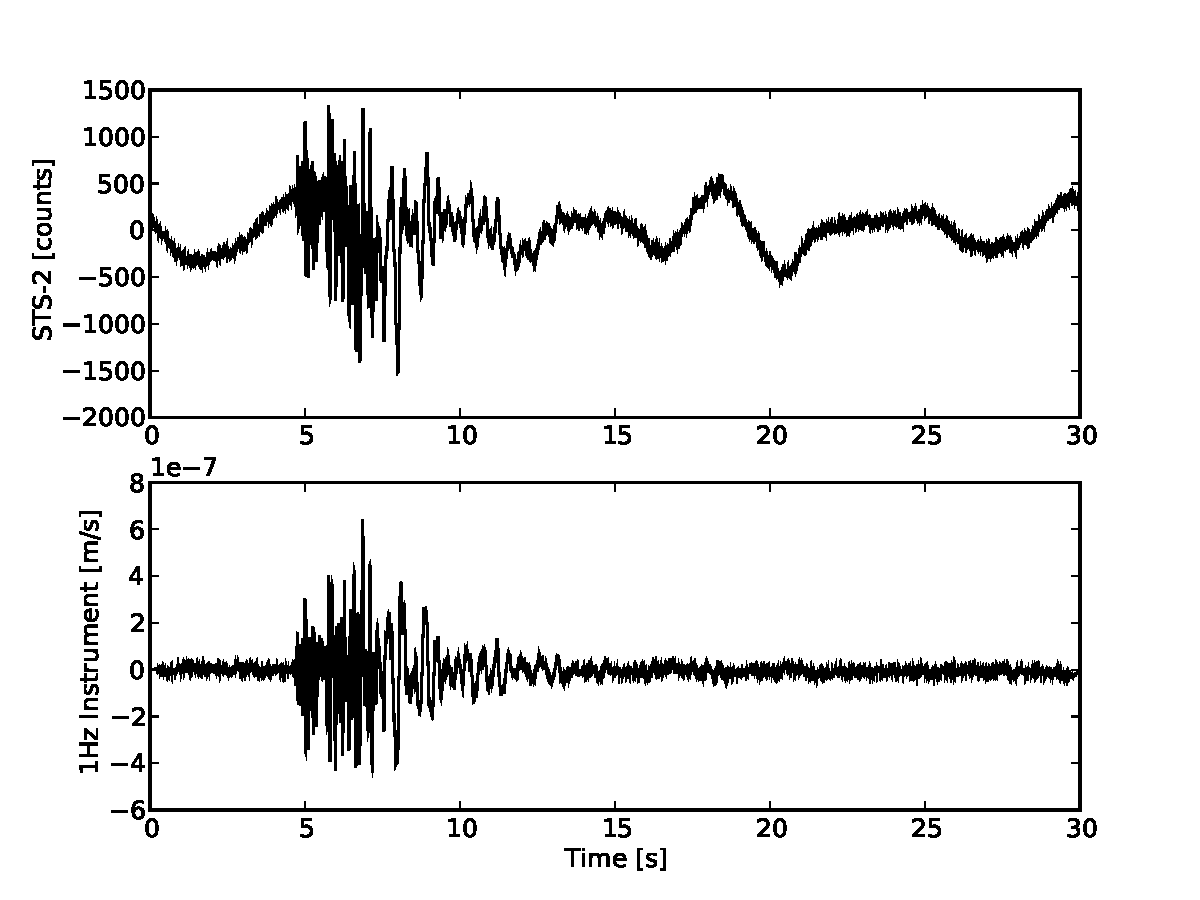
\includegraphics[height=.30\MyBoxWidth]{korrektur}\\[-3ex]
};
\end{tikzpicture}
	{\small
	\textbf{Figure~2}: Correction of a STS2 to a 1Hz instrument.
	} \\[.5\MyBoxVSep]
\end{center}

\begin{center}
\begin{tikzpicture}
\node[above right,text width=.45\MyBoxWidth]at(0cm,0cm){ 
\tiny
\centering
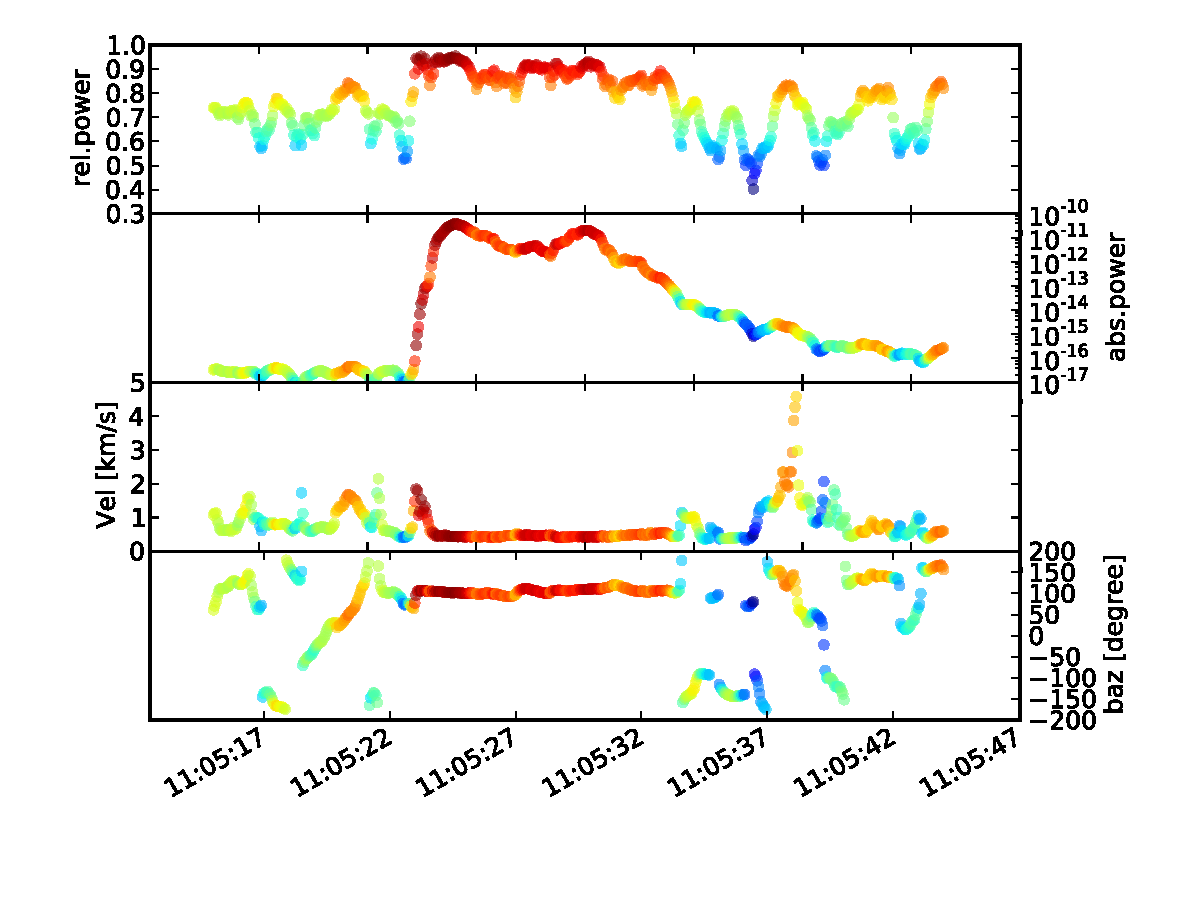
\includegraphics[height=.30\MyBoxWidth]{beamforming2}\\[-3ex]
};
\end{tikzpicture}
	{\small
	\textbf{Figure~3}: Output of a FK Analysis from blasting the AGFA skyscraper in Munich. Colors correspond to relative power.
	} \\[.5\MyBoxVSep]
\end{center}

\begin{center}
\begin{tikzpicture}
\node[above right,text width=.45\MyBoxWidth]at(0cm,0cm){ 
\tiny
\centering
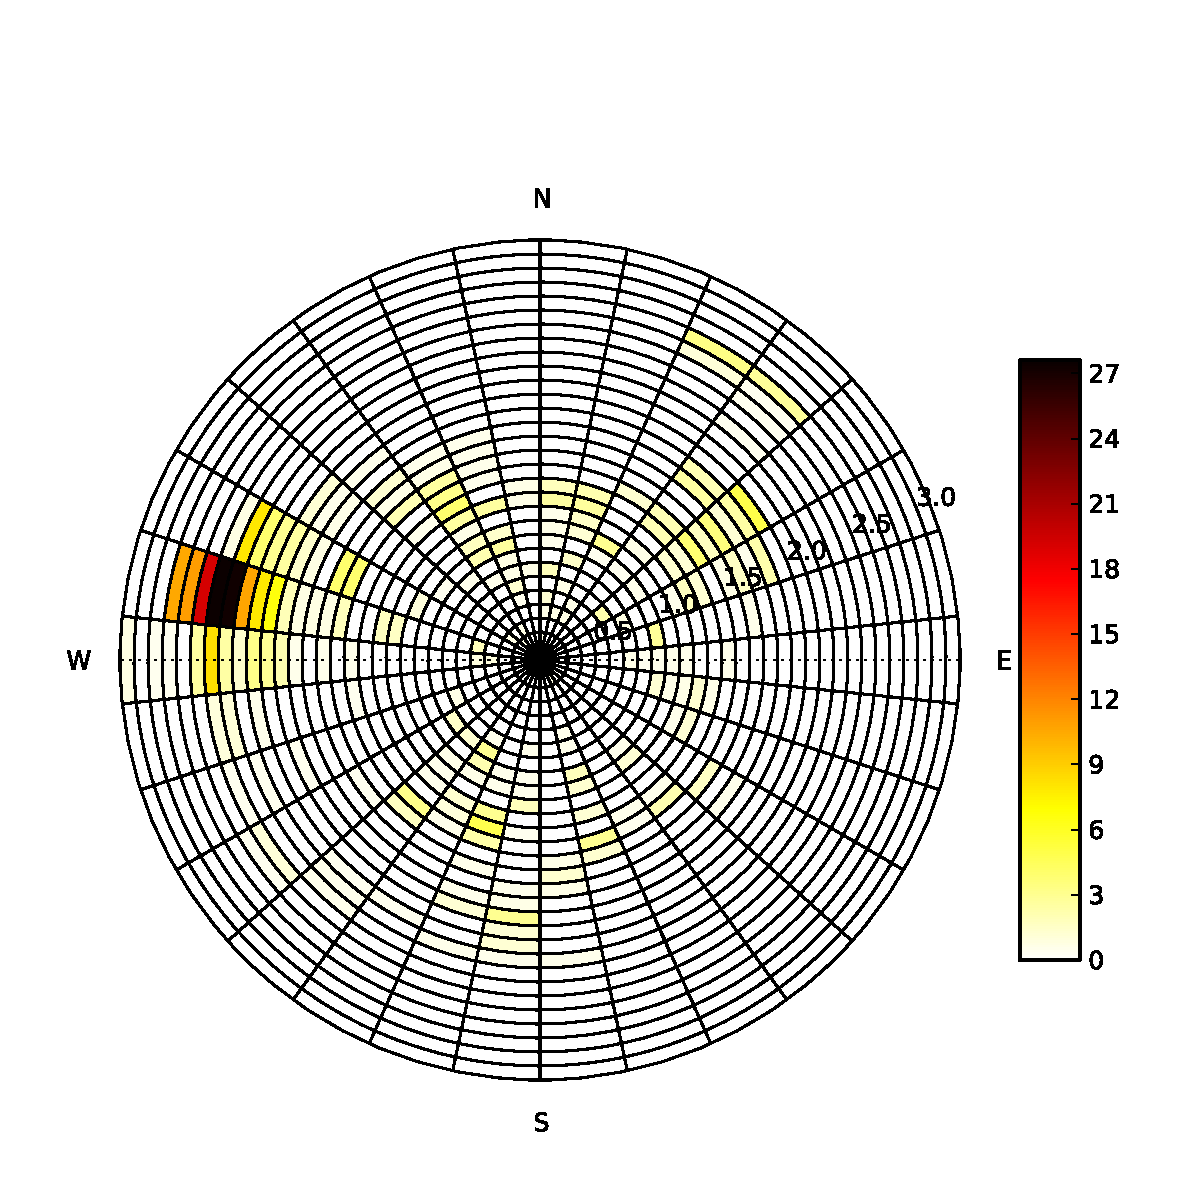
\includegraphics[height=.30\MyBoxWidth]{fkanalysis}\\[-3ex]
};
\end{tikzpicture}
	{\small
	\textbf{Figure~4}: Polar plot of the same FK Analysis.
	} \\[.5\MyBoxVSep]
\end{center}
\end{multicols}
}\vspace{\MyBoxVSep}

\end{multicols}
% First reduce the vertical spacing to zero and then expand again.
\vspace{-0.60cm}
\vspace{\MyBoxVSep}

% New width.
\setlength{\MyBoxWidth}{736.5mm}
% Single Large Box to take care of the example.
\MyBox[8em]{
\begin{multicols}{3}
\section*{Applications Using ObsPy}
Combining Python and ObsPy facilitates the development of applications ranging from little helper scripts to full blown platform-independent GUI applications with complex workflows.\\
This section highlights two GUI programs both based on Qt (qt.nokia.com) for the graphical representation. Both were developed in a matter of a few month and make use of ObsPy for the underlying internal data storage which in turn enables them to utilize ObsPy's routines for many commonly used tasks, e.g. filtering and instrument simulation and they instantly gain the ability to work with most commonly used waveform dataformats.\\
Other advanced third party Python modules that are easily integrated can take care of most processing and plotting needs so the programmer can focus on creating unique new features.\\
An up to date list of programs making use of ObsPy is available at www.obspy.org. A notable example is the newly developed version of \textbf{SeismicHandler} (www.seismic-handler.org) which is also represented at this meeting.
\columnbreak
\begin{center}
\begin{tikzpicture}
\node[above right,text width=.17\MyBoxWidth]at(0cm,0cm){ 
\tiny
\centering
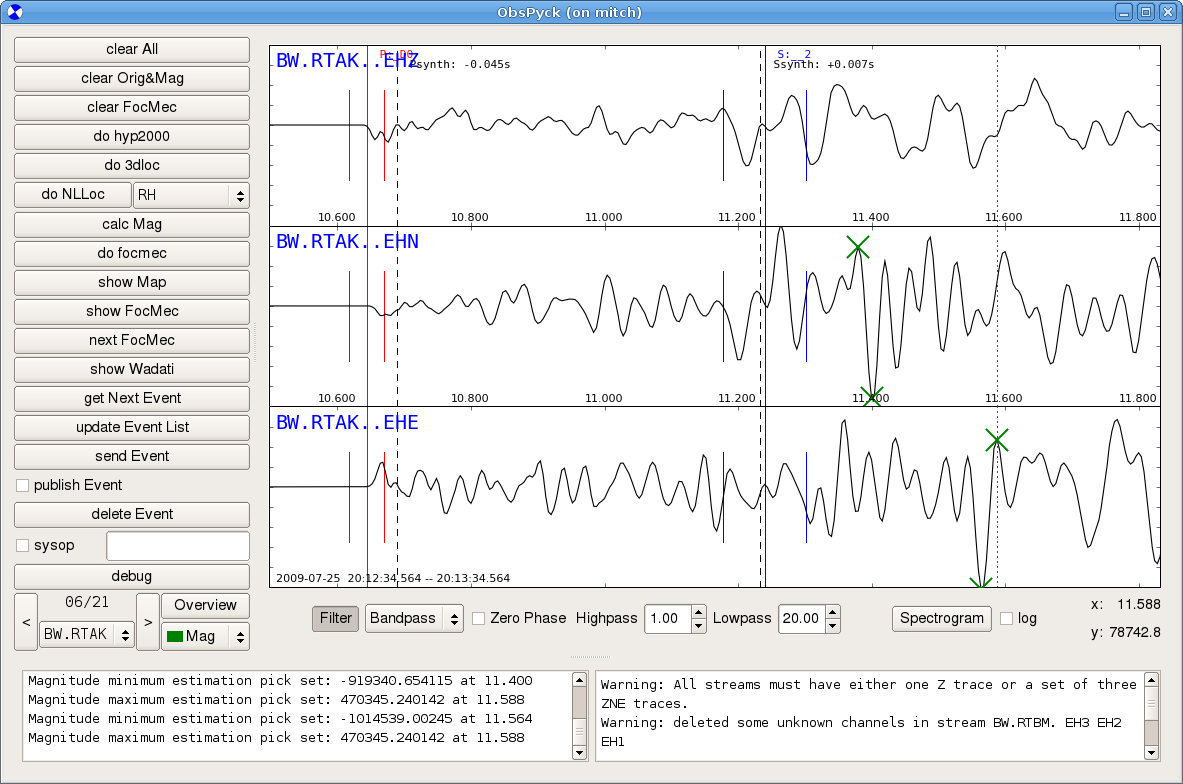
\includegraphics[height=.17\MyBoxWidth]{all_picks}\\[-3ex]
};
\end{tikzpicture}
{\newline \small \textbf{Figure~5}: ObsPyck
} \\[.5\MyBoxVSep]
\end{center}

\textbf{ObsPyck} is able to perform daily routine analysis at an observatory like phase picking and locating events. All data is read and written back to one central SeisHub database server and it just recently was extended to fetch data from ArcLink and Fissures servers to integrate external data into the localization process.
\columnbreak
\begin{center}
\begin{tikzpicture}
\node[above right,text width=.17\MyBoxWidth]at(0cm,0cm){ 
\tiny
\centering
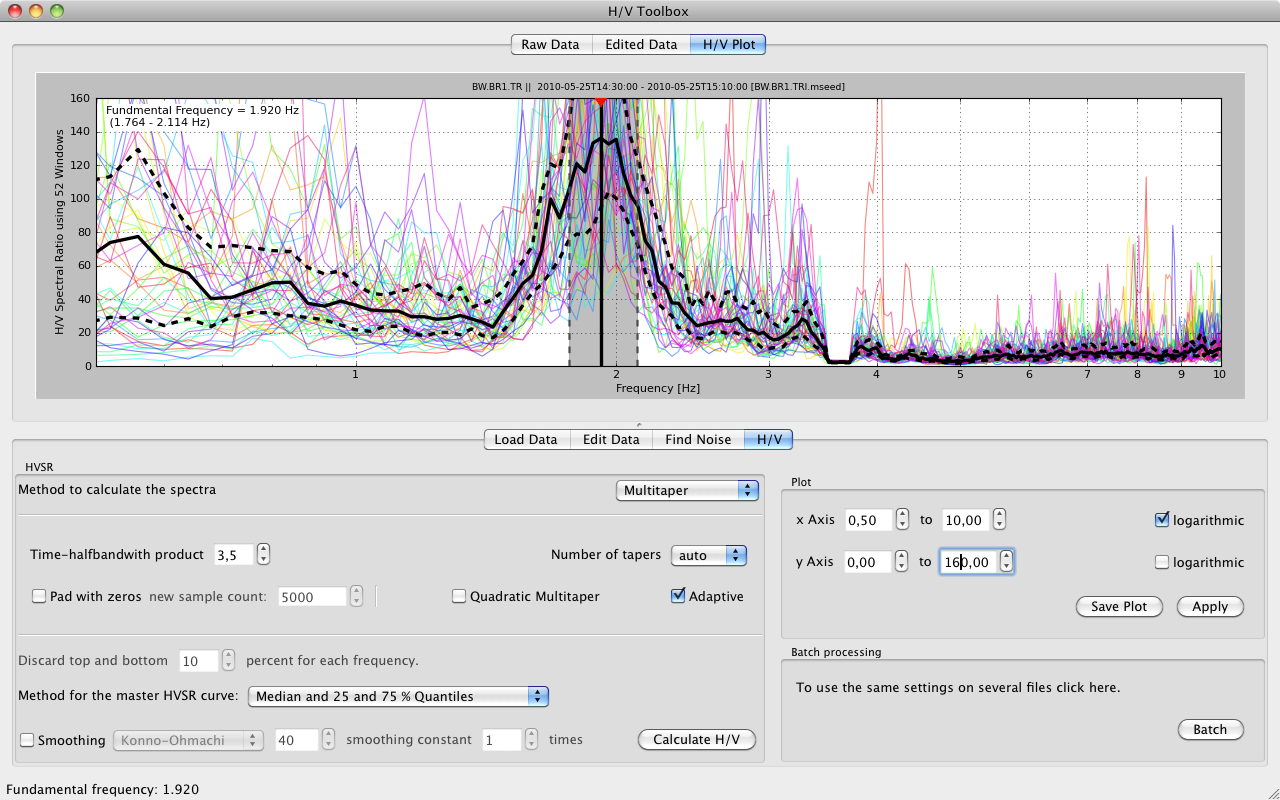
\includegraphics[height=.17\MyBoxWidth]{htovtoolbox}\\[-3ex]
};
\end{tikzpicture}
{\newline \small \textbf{Figure~6}: H/V Toolbox
} \\[.5\MyBoxVSep]
\end{center}
The \textbf{H/V Toolbox} handles the whole workflow for calculating horizontal to vertical spectral ratios (HVSR): From reading and preprocessing the data to the automated selection of appropriate time windows with little seismic activity to finally calculating the HVSR in an easy to use interface while giving visual feedback, step by step.




\end{multicols}
}

\setlength{\MyBoxWidth}{355mm}
\begin{multicols}{2}

\MyBox[8em]{
\section*{Further Information: http://www.obspy.org}
The homepage of the project \textbf{http://www.obspy.org} contains extensive \textbf{documentation}, tutorials, installation instructions for various platforms, and many more examples.
\newline
Contact the developers for support or feedback, to report bugs or to request a new feature. Contributions are more than welcome, see the developer links on the homepage if you are interested.
\newline

\underline{\textbf{Further functionality and information:}}
\begin{itemize}
\item \textbf{obspy.signal:} Filters, triggers, instrument correction, rotation, array analysis, beamforming.
\item \textbf{obspy.imaging:} Imaging spectrograms, beachballs and waveforms.
\item \textbf{Test-driven development (TDD):} TDD and automated unit tests are used throughout the ObsPy code base to ensure a high quality. Automated build bots test the most current ObsPy build on a daily basis on multiple platforms.
\end{itemize}
}
\columnbreak%\\

%
% Ninth box.
%
\MyBox[8em]{
\section*{Literature}
\vspace{2mm}
\bibliography{poster}{}
\bibliographystyle{plaindin}
}
\end{multicols}
\end{document}
